\chapter{自动加样系统机械臂的设计}
自动加样系统能够实现的一个基本功用是在空间内平将待检样品和反应试剂用送到反应瓶内,实现任意位置的准确定位并且尽量减少加样时间同时保证运动的平稳。因此,自动加样系统的加样机械臂的设计十分重要和关键。本部分完成对其系统结构的设计。
\section{加样机械臂结构类型的选定}
机械臂结构类型多种多样,不同工作场景所使用的机械臂结构形式千差万别。工业上广泛使用的机械臂结构主要有以下几种:

1.铰接式结构:该设计由多个旋转接头和工作臂组成,从简单的双链接结构到多($5-8$个以上)相互作用的铰接系统。一般地,该结构在笛卡尔坐标系下能够实现三个转动自由度。一般情况下,铰接结构越多,工作范围越大,机械臂运动也就越精确。铰接式机械臂通常用于装配,压铸,气焊,及喷涂等工作场景。其机械结构简图如\ref{fig:3-1}。

\begin{figure}[htbp!]
	\centering
	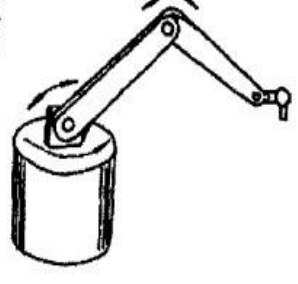
\includegraphics[height=6.5cm]{chap/figure/3-1.jpg}
	\caption{铰接式结构简图}
	\label{fig:3-1}
\end{figure}

2.笛卡尔式结构:该结构在笛卡尔坐标系下一般有三个平动自由度,它能实现机械臂在空间内沿着$X,Y,Z$方向平动从而到达坐标系中任意位置。笛卡尔式机械臂通常用于装载(卸载)工件,印刷电子电路板,材料表面处理等工作场景。该结构提供的工作空间大(可用于其它用途)、控制系统简单。其机械结构简图如\ref{fig:3-2}。

\begin{figure}[htbp!]
	\centering
	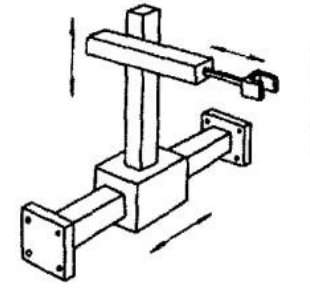
\includegraphics[height=6.5cm]{chap/figure/3-2.jpg}
	\caption{笛卡尔式结构简图}
	\label{fig:3-2}
\end{figure}

3.圆柱式结构:该结构在笛卡尔坐标系统能实现沿着$X,Y$方向平动和绕$Z$方向转动,机器臂可以移动到由圆柱体描述的体积内的任意位置。该结构在垂直方向上节省了空间,具有良好的刚性能承受较大的有效载荷,但由于其结构限制不能实现$360$度转动。其机械结构简图如\ref{fig:3-3}。

\begin{figure}[htbp!]
	\centering
	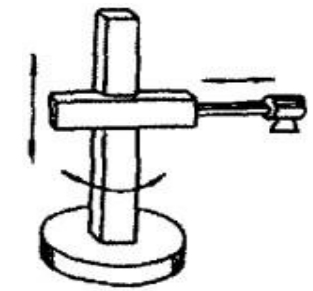
\includegraphics[height=6.5cm]{chap/figure/3-3.jpg}
	\caption{圆柱式结构简图}
	\label{fig:3-3}
\end{figure}

4.极坐标式结构:该结构在笛卡尔坐标系下一般能够实现两个旋转自由度和一个平动自由度。相比于圆柱式结构,它在空间内能实现$360$度的转动,并且在水平方向上的工作距离更长。其机械结构简图如\ref{fig:3-4}。

\begin{figure}[htbp!]
	\centering
	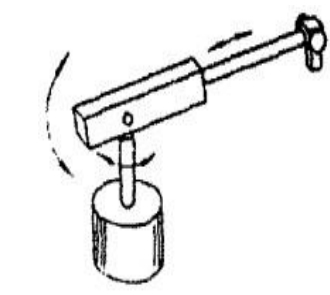
\includegraphics[height=6.5cm]{chap/figure/3-4.jpg}
	\caption{极坐标式结构简图}
	\label{fig:3-4}
\end{figure}

根据加样系统的功用和动作流程,加样机械臂要能够到达三维空间中的任意位置;加样多孔板需要放置在工作台上,要求工作台空间足够大;加样液在移送过程中不能有滴漏,要求加样机械臂运动平稳;取样、释样过程不能发生样品(试剂)出错现象,要求加样机械臂运动精度高。考虑以上要素,综合对比上述四种机械臂结构本文选用笛卡尔式结构,该结构能够提供较大的工作空间,控制易于实现,运动平稳且精度高。
\section{驱动方式的选定}

加样机械臂的运动状态是由其驱动系统决定的,它一般由两个部分组成:驱动机构和传动机构。驱动机构其实质可以视为一种可以将其它能量如气动能量、电能等转化为加样机械臂的动能的装置,并通过传动机构使得机械臂动作。根据动力源的不同,可以将其分为电力源、液压源和气压源三种驱动类型。

电力驱动:该方式利用电动机产生的力矩和力驱动机械臂进行动作,其具有速度调节范围广、控制精度高、运动平稳性高的特点,具有良好的的控制性和环境适应性。常用的电机驱动器包括直流伺服电机、交流伺服电机、步进电机等。

液压驱动:该方式利用液体产生的压力驱动机械臂进行动作,其具有动力大,无级调速,能实现高速的精度控制等特点。但供油回油等附加元件使其系统体积大,成本高,维修困难,易泄漏对环境极度不友好、。该驱动方式多用于矿山机械,重型设备等。

气压驱动:该方式利用气体产生的压力驱动机械臂进行动作,其具有响应快清洁无害,易维护等特点。但其运动稳定性差,功率小,噪声大、难以实现较高精度的位置和速度控制,多用于小功率驱动、运动精度要求低的场合。

自动加样系统在加样过程中进行多次重复加样,位置重复性要求好;加样系统必须具有一定的效率,短时间内完成较多的加样任务,速度响应要求要好;加样过程中,为保证测试结果的准确度取样要准,运动平稳性和精度要求高。要求其运动平稳性好,位置精度高;其部件模块不大、负载小;并且,自动加样系统一般多用于医院、科研机构等对噪声要求严苛的地方。比较上述三种驱动方式,本文选用电力驱动。

进一步地,电力驱动所用的驱动器通常有直流伺服电机、交流伺服电机、步进电机。对于伺服电机,其主要特点是马达或执行机构上装有传感器,传感器将命令执行结果经由伺服放大器传回控制中心,控制中心在比较执行结果和指令值之后再对执行结果进行反馈纠正以不断减小运动执行误差。可以实现转速可以精确控制,速度控制范围广,除了可以进行稳定平顺等速运转之外,还可以根据需求随时变更速度。然而,一般伺服电机采取的控制方式是闭环控制,闭环系统中机械部件的惯性、传动误差、变形刚度等问题使得控制极其复杂和困难。而步进电机不用配备转角编码器等设备,且不受输入和输出因素的影响也不受冲击和振动等环境因素的影响;由脉冲信号控制执行机构运动的距离和速度,在不失步运行时步距累积误差为0,不需要位置检出和速度检出的回授元件,所以步进电机的输出可以由单一的脉冲的输入来决定,因此就能达成精确的位置和速度控制。另外,可以通过位置传感器(如限位开关)来辅助位置和速度的控制。步进电机对比伺服电机一个难以匹敌的优点是它使得本设计的系统体积小,结构紧凑。综合控制成本和控制效果来看,本文选择步进电机作为$X$、$Y$、$Z$方向平动的驱动器。

\section{传动方式选定}
加样机械臂传动方式对加样精度、稳定性和响应的快速性都产生重要影响。机械系统中传动机构多种多样,本文初步选定将步进电机的回转运动转换成直线运动的滚珠丝杠螺母传动和同步带。

滚珠丝杠螺母传动机构与一般的丝杠螺母副一致,但其在丝杠和螺母之间增加了滚珠。丝杠转动的同时滚珠也会在螺纹滚道里转动,滚珠又将运动传递给螺母,通过一系列的动作将转动量变换成平动量。滚珠丝杠螺母传动机构的传递的效率高,摩擦损失小,传动精度高但是其结构复杂、难以加工、制造困难;并且滚珠丝杠螺母机构需要润滑和密封机构以提高其工作效率和寿命。同步带传动是带传动和齿轮传动的有机结合体,兼备二者的优点。同步带的内周表面制有等距的距齿。工作时,利用带与带轮齿之间的啮合关系传递运动\supercite{bib7}。同步带的传动比准确且恒定,最吸引的一个优点是带的缓冲吸振特性使其传动平稳,结构紧凑,不需要密封和润滑维护方便,并且重量小,传动能量利用效率高,刚度影响因素少。

加样机械臂的传动比要求较高,传动过程不能发生干涉现象,尽量降低回程误差以提高传动精度,故选取同步带作为传动机构。此外,为保证加样过程中运动的平稳性和高精度,导性机构本设计采用滚动直线导轨。滚动直线导轨以适当滚珠放入滑块和导轨之间,这种设计使得滚动摩擦代替滑动摩擦从而减低了摩擦阻力,实现了高定位精度和重复精度。


\section{加样机械臂机械结构的设计}
本小结在以上分析的基础上进行笛卡尔式加样机械臂的结构绘制。经过分析可知,加样机械臂包括步进电机,同步带,滚动直线导轨

加样系统整体布局如图\ref{fig:3-5}
\begin{figure}[htbp!]
	\centering
	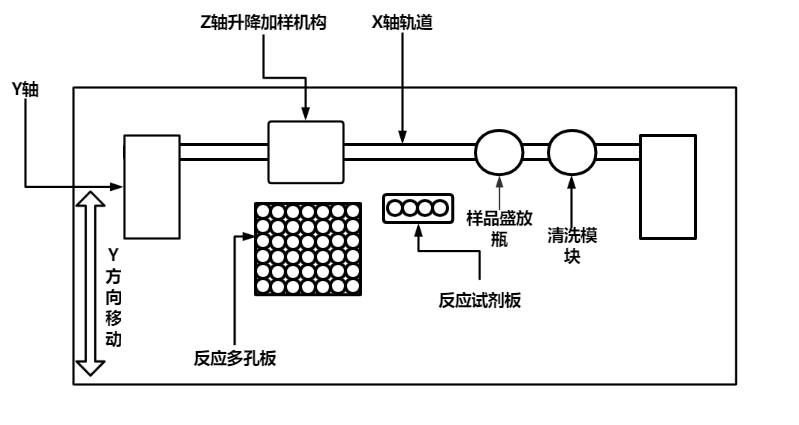
\includegraphics[height=8.5cm]{chap/figure/0.jpg}
	\caption{加样系统整体布局简图}
	\label{fig:3-5}
\end{figure}












































